\chapter{Exponential Functions, Logarithms and e}
\author{Nithin}

\section{Bacterial Growth on the Human Body}
\begin{itemize}
  \item Our skin (and other areas like the mouth, nose, and intestines) hosts hundreds of thousands of microscopic organisms.
  \item In fact, bacterial cells in our body outnumber our own cells.
  \item While some bacteria can cause illness, many are essential for our health.
  \item Bacteria reproduce through binary fission—each cell splits into two.
  \item Under ideal conditions, a single bacterium doubling every hour can lead to over 1,000 cells in 10 hours and more than 16 million in 24 hours.
\end{itemize}

\subsection{Bacterial Growth Over Time}
\begin{table}[ht]
  \centering
  \begin{tabular}{c|ccccccccccc}
    \textbf{Hour} & 0 & 1 & 2 & 3 & 4 & 5 & 6 & 7 & 8 & 9 & 10 \\ \hline
    \textbf{Bacteria} & 1 & 2 & 4 & 8 & 16 & 32 & 64 & 128 & 256 & 512 & 1024 \\
  \end{tabular}
  \caption{Bacterial cell count doubling every hour.}
\end{table}

\section{Population Growth in India}
\begin{itemize}
  \item India is the second most populous country, with about 1.39 billion people in 2021.
  \item Its population grows at an annual rate of roughly 1.2\%.
  \item If this trend continues, India's population is projected to exceed China’s by 2027.
  \item While rapid population increases are often described as "exponential," in mathematics the term has a very precise meaning.
\end{itemize}

\section{Defining Exponential Growth}
\begin{itemize}
  \item \textbf{Percentage Change:}
  \begin{itemize}
    \item refers to a change based on a percent of the original amount
  \end{itemize}
  \item \textbf{Exponential Growth:}
    \begin{itemize}
      \item refers to an increase based on a constant multiplicative rate of change over equal increments of time, that is, a percent increase of the original amount over time.
      \item For example, if a quantity doubles each period, that is a 100\% increase per period.
    \end{itemize}
  \item \textbf{Linear Growth:}
    \begin{itemize}
      \item The original value increases by a fixed \textbf{amount} (additive rate) over equal time intervals.
    \end{itemize}
    \item \textbf{Exponent Decay:}
    \begin{itemize}
      \item refers to a decrease based on a constant multiplicative rate of change over equal increments of time, that is, a percent decrease of the original amount over time.
    \end{itemize}
\end{itemize}

\section{Exponential Function and Its Behavior}
Suppose \(b>0\) with \(b\neq 1\). Then the \emph{exponential function} with base \(b\) is defined by
\[ f(x)=b^x. \]
For example, if \(b=2\), then \(f(x)=2^x\). (Note that \(2^x\) is different from \(x^2\).)

\subsection{Behavior (for \(b>1\))}
\begin{itemize}
  \item \textbf{Domain:} All real numbers, \(\mathbb{R}\).
  \item \textbf{Range:} All positive numbers, \((0,\infty)\).
  \item \(f(x)=b^x\) is an \emph{increasing} function.
  \item \(b^x\) becomes very large as \(x\) increases.
  \item \(b^x\) approaches \(0\) as \(x\) becomes very negative.
\end{itemize}

\section{Comparing Exponential and Linear Growth}
\begin{table}[ht]
  \centering
  \begin{tabular}{c|c|c}
    \(x\) & \(f(x)=2^x\) & \(g(x)=2x\) \\ \hline
    0 & 1 & 0 \\
    1 & 2 & 2 \\
    2 & 4 & 4 \\
    3 & 8 & 6 \\
    4 & 16 & 8 \\
  \end{tabular}
  \caption{Exponential vs. Linear Growth.}
\end{table}
\begin{itemize}
  \item Linear growth (e.g., \(g(x)=2x\)) increases by a constant amount (2) for each increase in \(x\), that is, it is adding or subtracting a constant value. A constant amount \( \rightarrow \) linear growth or additive growth.
  \item Exponential growth (e.g., \(f(x)=2^x\)) increases by a constant factor (2) for each increase in \(x\), that is, it is multiplying or dividing by a constant value. A constant factor \( \rightarrow \) exponential growth or multiplicative growth.
\end{itemize}

\section{Example: The Function \(f(x)=2^x\)}
\begin{table}[ht]
  \centering
  \begin{tabular}{|c|c|c|c|c|c|c|c|}
    \hline
    \(x\)      & -3 & -2 & -1 & 0 & 1 & 2 & 3 \\ \hline
    \(2^x\) & \(2^{-3}=\frac{1}{8}\) & \(2^{-2}=\frac{1}{4}\) & \(2^{-1}=\frac{1}{2}\) & \(2^0=1\) & \(2^1=2\) & \(2^2=4\) & \(2^3=8\) \\ \hline
  \end{tabular}
  \caption{Exponential values of \(2^x\) for \(x=-3,\dots,3\).}
\end{table}
\textbf{Observation:} As \(x\) increases by 1, the output of \(2^x\) doubles, clearly illustrating exponential growth.

\section{Algebraic Properties of Exponents}
Let \(a, b > 0\) and \(x, y \in \mathbb{R}\). Then:
\begin{itemize}
  \item \(b^x \cdot b^y = b^{x+y}\)
  \item \((b^x)^y = b^{xy}\)
  \item \(a^x \cdot b^x = (ab)^x\)
  \item \(b^0 = 1\)
  \item \(b^{-x} = \dfrac{1}{b^x}\)
  \item \(\dfrac{b^x}{b^y} = b^{x-y}\)
  \item \(\dfrac{a^x}{b^x} = \Bigl(\dfrac{a}{b}\Bigr)^x\)
\end{itemize}

\subsection{Exponent Graph}
\begin{figure}
\centering
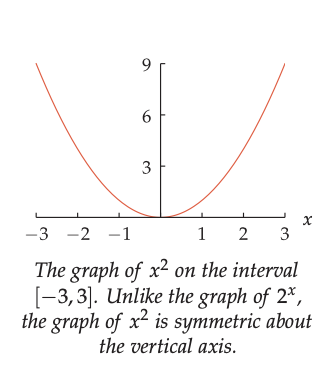
\includegraphics[scale=0.3]{pics/exp-vs-poly1.png}
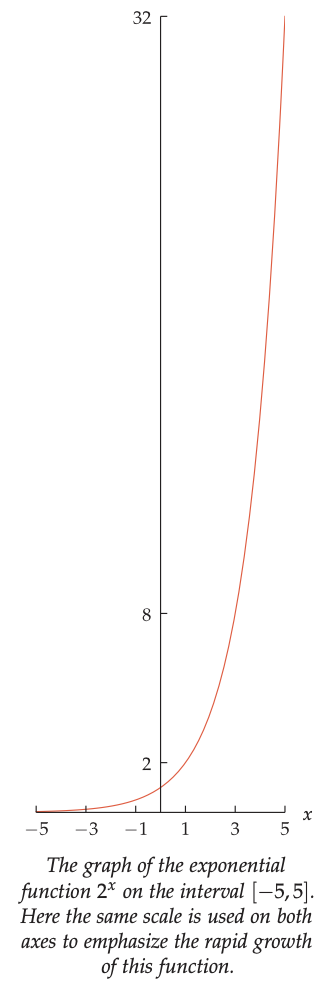
\includegraphics[scale=0.2]{pics/exp-vs-poly2.png}
\end{figure}

\section{Logarithm}
Suppose \(b\) and \(y\) are positive numbers with \(b\neq 1\).
\begin{itemize}
  \item The logarithm base \(b\) of \(y\), denoted \(\log_b y\), is defined as the unique number \(x\) such that
  \[ b^x = y. \]
  \item  Short Version
  \[ \log_b y = x \quad \text{means} \quad b^x = y. \]
\end{itemize}

\subsection{Logarithm of 1 and the Base}
Let \(b>0\) with \(b\neq 1\). Then:
\begin{itemize}
  \item \(\log_b 1 = 0\) because \(b^0 = 1\),
  \item \(\log_b b = 1\) because \(b^1 = b\).
\end{itemize}

\subsection{Logarithm as an Inverse Function}
Suppose \(b\) is a positive number with \(b \neq 1\) and the exponential function \(f\) is defined by
\[ f(x) = b^x. \]
Then the inverse function \(f^{-1}\) is given by
\[ f^{-1}(y) = \log_b y. \]

\subsection{Inverse Properties of Logarithms - Summary}
\begin{itemize}
  \item \textbf{Inverse Relationship:}
    \begin{itemize}
      \item \(\log_b x\) is the inverse of \(b^x\).
      \item Flipping the graph of \(b^x\) across the line \(y=x\) yields the graph of \(\log_b x\).
    \end{itemize}
  \item \textbf{Monotonicity:}
    \begin{itemize}
      \item For \(b>1\), \(b^x\) is increasing, so \(\log_b x\) is also increasing.
    \end{itemize}
  \item \textbf{Key Equations:}
    \begin{itemize}
      \item \(b^{\log_b y} = y\)
      \item \(\log_b (b^x) = x\)
    \end{itemize}
  \item \textbf{Function-Inverse Properties:}
    \begin{itemize}
      \item These can be written as \((f \circ f^{-1})(y) = y\) and \((f^{-1} \circ f)(x) = x\).
    \end{itemize}
  \item \textbf{Understanding:}
    \begin{itemize}
      \item These properties are fundamental to the relationship between exponential and logarithmic functions.
    \end{itemize}
\end{itemize}

\subsection{Logarithm of a Power}
If \(b\) and \(y\) are positive numbers, with \(b \neq 1\), and \(t\) is a real number, then
\[ \log_b\left(y^t\right) = t \log_b y. \]

\section{Radioactive Decay}
If a radioactive isotope has half-life \(h\), then the function modeling the number of atoms in a sample of this isotope is
\[ a(t) = a_{0}2^{-t/h}\]
where \(a_{0}\) is the number of atoms of the isotope in the sample at time \(0\).

\section{Exponential Growth}
\subsection{A story}
A mathematician in ancient India invented the game of chess. Filled with gratitude for the remarkable entertainment of this game, the king offered themathematician anything he wanted. The king expected the mathematician to ask for rare jewels or a majestic palace. But the mathematician asked only that he be given one grain of rice for the first square on a chessboard, plus two grains of rice for the next square, plus four grains for the next square, and so on, doubling the amount for each square, until the 64th square on an 8-by-8 chessboard had been reached. The king was pleasantly surprised that the mathematician had asked for such a modest reward. A bag of rice was opened, and first 1 grain was set aside, then 2, then 4, then 8, and so on. As the eighth square was reached, 128 grains of rice were counted out. The king was secretly delighted to be paying such a small reward and also wondering at the foolishness of the mathematician.

As the 16th square was reached, 32,768 grains of rice were counted out—this was a small part of a bag of rice. But the 21st square required a full bag of rice, and the 24th square required eight bags of rice. This was more than the king had expected. However, it was a trivial amount because the royal granary contained about 200,000 bags of rice to feed the kingdom during the coming winter. As the 31st square was reached, over a thousand bags of rice were required and were delivered from the royal granary. Now the king was worried. By the 37th square, the royal granary was two-thirds empty. The 38th square would have required more bags of rice than were left. The king then stopped the process and ordered that the mathematician's head be chopped off as a warning about the greed induced by exponential growth.

\subsection{Mathematical analysis}
\begin{itemize}
  \item \(64^{th}\) square requires \( 2^{63} \) grains \(\approx\) \(2^{3}* (2^{10})^{6} = 8*(10^{3})^{6} = 8*10^{18} \approx 10^{19} \)
  \item if one large bag = \(10^{6} \) grains of rice , then total bags = \(10^{19}/10^{6} \)
  \item In 2025 India's population is \(\approx 1 * 10^{9} \)
\end{itemize}

A function \(f\) is said to have \textbf{exponential growth} if \(f(x) = cb^{kx} \) where
\(c\) and \(k\) are positive numbers and \(b > 1\).
\begin{itemize}
  \item \(f(x) > p(x)\)  where \(f\) is exponenetial and \(p\) is polynomial for sufficiently large \(x\)
  \item \(2^{x} > x^{1000} \)  \(\forall \;	kWidget x > 13747 \)
  \item A function \(f\) has exponential growth if and only if the graph of \(\log f(x)\) is a line with a positive slope
\end{itemize}

\section{Population Growth}
\[ p(t) = p_0\,e^{rt} \]
\begin{itemize}
  \item \(p_0\): initial population
  \item \(r\): constant per-capita growth rate
  \item Assumes unlimited resources \rightarrow population grows without bound
  \item Populations of various organisms, ranging from bacteria to humans, often exhibit exponential growth
\end{itemize}

\subsection{Population Growth: Example}
Suppose a colony of bacteria in a petri dish has 700 cells at 1 pm. These bacteria reproduce at a rate that leads to doubling every three hours. How many bacteria cells will be in the petri dish at 9 pm on the same day?
\[ p(t) = p_{0}2^{t/3} \implies 700 \cdot 2^{8/3} \]

\subsection{Exponential growth and doubling}
If a population doubles every \( d \) time units, then the function \( p \) modeling this population growth is given by the formula
\[ p(t) = p_{0} \cdot 2^{(t-t_{0})/d} \]
where \(p_{0}\) is the population at time \(t_{0}\).

\section{Compound Interest}
\begin{figure}
  
\includegraphics[scale=0.3]{pics/CI-comic.png}
\end{figure}

\subsection{Example}
Suppose you deposit \(8000\) in a bank account that pays \(5\%\) annual interest. Assume the bank pays interest once per year at the end of the year, and that each year you place the interest in a cookie jar for safekeeping.
\begin{enumerate}
  \item  How much will you have (original amount plus interest) at the end of two years?
  \item How much will you have (original amount plus interest) at the end of t years?
\end{enumerate}
Interest per year \( = 8000*0.05 = 400 \). For 2 years \( = 400*2 = 800\).
After \(t\) years \(= 8000 + 8000*0.05*t = 8000(1+0.05t)\).

\subsection{Simple Interest}
If interest is paid once per year at the annual rate of \(r\), with no interest paid on the interest, then after \(t\) years
an initial amount \(P\) grows to
\[ P(t) = P_{0}(1 + rt) \]

\subsection{Example}
Suppose you deposit \(8000\) in a bank account that pays \(5\%\) annual interest. Assume the bank pays interest once per year at the end of the year, and that each year the interest is deposited in the bank account.
\begin{enumerate}
  \item How much will you have at the end of one year?
  \item How much will you have at the end of two years?
  \item How much will you have at the end of t years?
\end{enumerate}
\begin{enumerate}
  \item  At the end of an year \( =  8000 + 8000*0.05  = 8400 \implies 8000(1+0.05)
  \item  At the end of 2 year \( = 8400 + 8400*0.05 \implies 8400( 1 + 0.05) = 8000(1.05)^{2} \)
  \item  At the end of \(t\) years \(= 8000(1.05)^{t}\)
\end{enumerate}

\subsection{SI vs CI}
\begin{figure}
  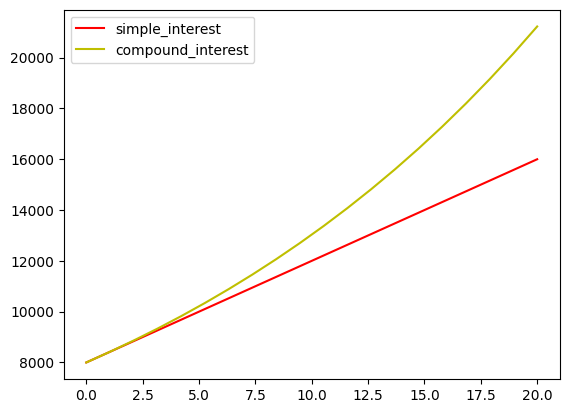
\includegraphics[scale=0.5]{pics/SI_vs_CI.png}
\end{figure}

\subsection{Example}
\begin{itemize}
  \item Interest is often compounded more than once per year
  \item In the above example,if the interest is compunded twice an year means instead of \(5\%\) being paid every year the interest comes as two payments of \(2.5\%\) each year with each payment made at the end of every 6 months
\end{itemize}
Suppose you deposit \(8000\) in a bank account that pays \(5\%\) annual interest, compounded twice per year. How much will you have at the end of one year?
\begin{itemize}
  \item At the end of 6 months \(= 8000(1+.025) \)
  \item At the end of 1 year = \( (8000*1.025)(1.025) = (8000*1.05/2)^2 \)
  \item At the end of t years = \(8000*(1+\frac{0.05}{2})^{2*t} \)
\end{itemize}

\subsection{Compound Interest}
If the interest is compounded \(n\) times per year at annual interest rate \(r\) then after \(t\) years an initial amount of \(P_{0}\) grows to
\[P(t) = P_{0}(1+\frac{r}{n})^{nt}\]

\section{\( e \)}
\begin{figure}
  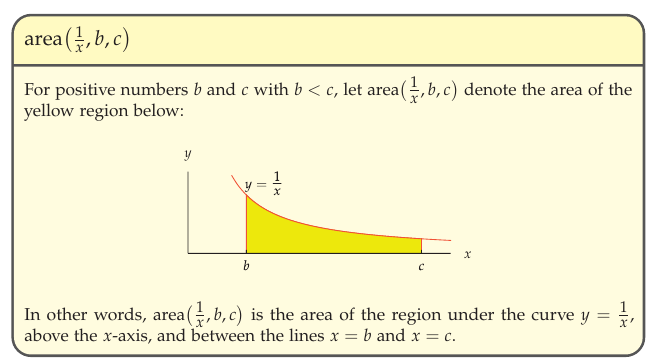
\includegraphics[scale=0.5]{pics/e_1.png}
\end{figure}

\subsection{area\((\frac{1}{x},1,2) < 1 \) }
\begin{figure}
  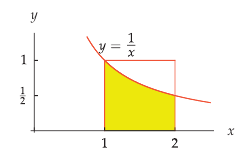
\includegraphics[scale=0.8]{pics/e_2.png}
\end{figure}
\begin{itemize}
  \item The area of the rectangle between \(x=1\) and \(x=2\) is \(1\)
  \item The yellow region lies inside the rectangle and the area of the yellow region is less than \(1\)
\end{itemize}

\subsection{area\((\frac{1}{x},1,3) > 1 \) }
\begin{figure}
  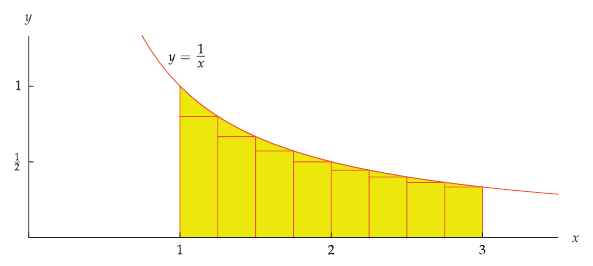
\includegraphics[scale=0.28]{pics/e_3.png}
\end{figure}
\begin{itemize}
  \item Interval \([1, 3]\) divided into 8 equal parts; each has width \(\frac{1}{4}\).
  \item Heights are calculated using \(f(x) = \frac{1}{x}\) at left endpoints of subintervals.
  \item First three rectangles:
  \begin{itemize}
      \item 1st: Height = \(\frac{1}{\frac{5}{4}} = \frac{4}{5}\), Area = \(\frac{1}{4} \cdot \frac{4}{5} = \frac{1}{5}\)
      \item 2nd: Height = \(\frac{1}{\frac{7}{4}} = \frac{4}{7}\), Area = \(\frac{1}{4} \cdot \frac{4}{7} = \frac{1}{7}\)
      \item 3rd: Height = \(\frac{1}{\frac{9}{4}} = \frac{4}{9}\), Area = \(\frac{1}{4} \cdot \frac{4}{9} = \frac{1}{9}\)
  \end{itemize}
  \item Guess for all areas: \(\frac{1}{5}, \frac{1}{6}, \frac{1}{7}, \dots, \frac{1}{12}\)
  \item Total area: \(\sum_{k=5}^{12} \frac{1}{k} = \frac{28271}{27720} > 1\)
\end{itemize}

\subsection{Defining \(e\)}
\begin{itemize}
  \item Consider the area under \(y = \frac{1}{x}\) from \(1\) to \(c\).
  \item area\((\frac{1}{x},1,2^{2})\) = \(2*\text{area}(\frac{1}{x},1,2)\)
  \item area\((\frac{1}{x},1,3^{2})\) = \(2*\text{area}(\frac{1}{x},1,3)\)
  \item area\((\frac{1}{x},1,2^{3})\) = \(3*\text{area}(\frac{1}{x},1,2)\)
  \item In general, area\((\frac{1}{x},1,c^{t}) = t*\text{area}(\frac{1}{x},1,c)\) for every \(t>0\) and \(c>1\).
\end{itemize}
\begin{tabular}{|c|c|}
  \hline
  \( c \) & \( \text{Area }( \frac{1}{x},1, c )\) \\ \hline
  2 & 0.693147 \\
  3 & 1.098612 \\
  4 & 1.386294 \\
  5 & 1.609438 \\
  6 & 1.791759 \\
  7 & 1.945910 \\
  8 & 2.079442 \\
  9 & 2.197225 \\
  \hline
\end{tabular}

\begin{figure}
  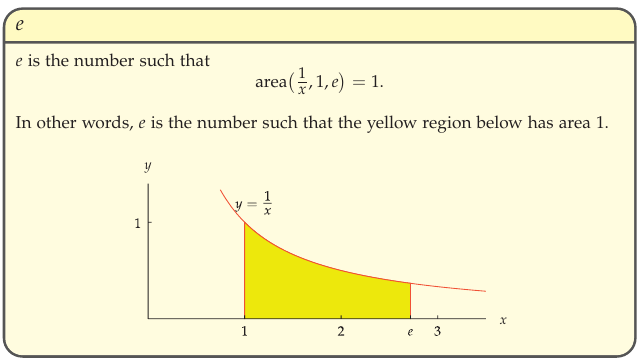
\includegraphics[scale=0.5]{pics/e_4.png}
\end{figure}

\subsection{Irrationality of \(e\)}
\begin{itemize}
  \item The number \(e\) is irrational.
  \item Here is a 40-digit approximation of \(e\):
  \item \(e \approx 2.718281828459045235360287471352662497757\)
\end{itemize}

\subsection{Defining the Natural Logarithm}
area\((\frac{1}{x},1,c^{t}) = t*\text{area}(\frac{1}{x},1,c) \)
\begin{itemize}
  \item The formula resembles the bhaviour of logarithms.
  \item Thus, area uner the curve \(y = \frac{1}{x}\) is connected with a logarithm
\end{itemize}
\[\text{area}(\frac{1}{x},1,e) = 1 \]
\[\text{area}(\frac{1}{x},1,e^{t}) = t \]
Assume \(t = \log_e c\) (the natural logarithm of \(c\)). Then we have
\[\text{area}(\frac{1}{x},1,c) = \text{area}(\frac{1}{x},1,e^{\log_e c}) = \log_e c\]

\subsection{Natural Logarithm}
The natural logarithm, denoted \(\ln\), is defined as follows:
\[ \ln c = \log_e c \]
for \(c > 1\).
\begin{figure}
  \centering
  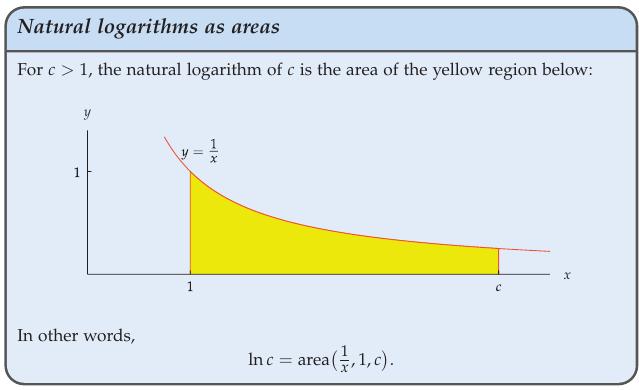
\includegraphics[scale=0.35]{pics/e_5.png}
\end{figure}

\subsection{The exponenetial function}
The \textbf{exponential function} is the function \(f\) defined by
\[ f(x) = e^{x} \]
for all \(x \in \mathbb{R}\).
\begin{itemize}
    \item The exponential function with base \( b \) is defined as \( b^x \).
    \item If no base is mentioned, assume the base is \( e \).
    \item The graph of \( e^x \) resembles \( 2^x \), \( 3^x \), etc., for \( b > 1 \).
    \item The function \(b^{x}\) is defined as \( b^{x} = e^{\ln b^{x}} \)
\end{itemize}

\subsection{Properties of the Natural Logarithm}
\begin{itemize}
  \item \(\ln 1 = 0\)
  \item \(\ln e = 1\)
  \item \(\ln e^{x} = x\)
  \item \(e^{\ln x} = x\) for \(x > 0\)
  \item \(\ln(ab) = \ln a + \ln b\)
  \item \(\ln\left(\frac{a}{b}\right) = \ln a - \ln b\)
  \item \(\ln(a^{b}) = b \cdot \ln a\)
  \item \(\ln\left(\frac{1}{a}\right) = -\ln a\)
  \item \(\ln a < \ln b\) if and only if \(a < b\) for \(a, b > 0\)
  \item \(\ln a = \ln b\) if and only if \(a = b\) for \(a, b > 0\)
  \item \(\ln a > 0\) if and only if \(a > 1\)
  \item \(\ln a < 0\) if and only if \(0 < a < 1\)
  \item \(\ln a = 0\) if and only if \(a = 1\)
\end{itemize}

\subsection{Values of \(t\) and \(\ln(1+t)\)}
\begin{table}[]
  \centering
  \begin{tabular}{|c|c|}
    \hline
    \(t\) & \(\ln(1+t)\) \\ \hline
    0.05 & 0.04879 \\
    0.005 & 0.00499 \\
    0.0005 & 0.00050 \\
    0.00005 & 0.00005 \\
    -0.05 & -0.05129 \\
    -0.005 & -0.00501 \\
    -0.0005 & -0.00050 \\
    -0.00005 & -0.00005 \\
    \hline
  \end{tabular}
  \caption{Table of \(t\) and \(\ln(1+t)\) for positive and negative values of \(t\).}
\end{table}

\subsection{\(y = \ln(1+t)\) as area under the curve \(y = \frac{1}{x}\)}
\begin{figure}
  \centering
  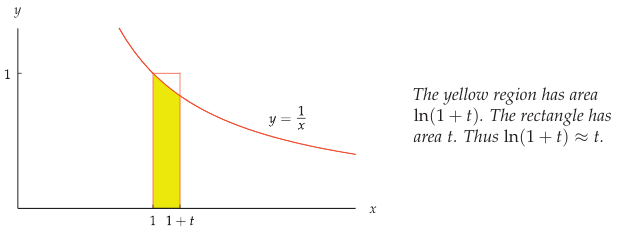
\includegraphics[scale=0.5]{pics/e_6.png}
\end{figure}
\begin{itemize}
  \item for small values of \(t\), the area rectangle becomes very small and it approximates the curve \(y = \frac{1}{x}\) very closely.
\end{itemize}

\subsection{The Exponential Function and the Natural Logarithm}
\subsubsection{Approximation of the Natural Logarithm}
if \(t\) is a small positive number, then
\[ \ln(1+t) \approx t \]

\subsection{Inequalites Involving the Natural Logarithm}
\begin{figure}
  \centering
  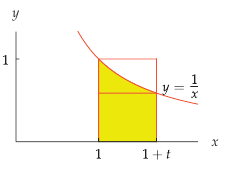
\includegraphics[scale=0.5]{pics/e_7.png}
\end{figure}
\begin{itemize}
  \item The area of the big rectangle is \( t * 1 = t \).
  \item Ther area of the smaller rectangle is \( t * \frac{1}{1+t} \).
  \item the area of the yellow region is \(   \frac{t}{1+t}  < \ln(1+t) < t \)
\end{itemize}

\subsection{Approximation of the exponential function for small \(x\)}
\begin{itemize}
  \item \(\ln(1+x) \approx x\ \implies e^{x} \approx e^{\ln(1+x)}  \implies e^{x} \approx 1 + x\)
\end{itemize}
If \(x\) is a small positive number, then
\[ e^{x} \approx 1 + x \]

\subsection{Approximation of the exponential function for large \(x\)}
\begin{itemize}
  \item If \(r << x\) then \(\frac{r}{x}\) is small \(\implies \left( e^{\frac{r}{x}}\right) \approx 1 + \frac{r}{x}\)
  \item \(e^{r} \approx \left(1+\frac{r}{x}\right)^{x} \)
\end{itemize}
If \(x\) is a large positive number and is much larger than \(|r|\), then
\[ \left(1+\frac{r}{x}\right)^{x} \approx e^{r} \]

\subsection{Estimate \(1.00002^{40}\)}
\[ 1.00002^{40} = \left(1 + 0.00002\right)^{40} = \left(1 + \frac{40*0.00002}{40} \right)^{40} = \left(1 + \frac{0.0008}{40} \right)^{40} \]\[ \approx e^{0.0008}\]
\[\approx 1 + 0.0008 = 1.0008 \]

\subsection{\( \left( 1 + t
ight)^{n}\)}
\( \left( 1 + t
ight)^{n} = \left(1 + \frac{nt}{n}\right)^{n} \approx e^{nt} \approx  1 + nt  \)
Suppose \(t\) and \(n\) are numbers such that \(|t|\) and \(|nt|\) are small. Then
\[ \left(1+t
ight)^{n} \approx 1 + nt \]

\subsection{Proof of area\( \left( \frac{1}{x}, 1, c^{t} \right) \) = \(t*\text{area}(\frac{1}{x}, 1, c)\)}
\begin{figure}
  \centering
  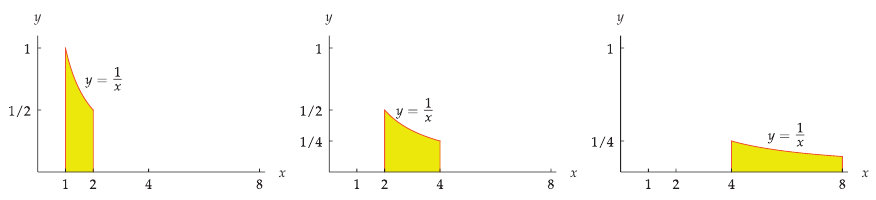
\includegraphics[scale=0.3]{pics/e_8.png}
\end{figure}
\begin{itemize}
  \item Applying the Area Stretch Theorem:
  \begin{itemize}
    \item The area under the curve in the left  = \(2*\frac{1}{2}\) times the area of the curve in the centre because the center curve can be obtained by stretching horizontally by \(2\) and verticall y by \(\frac{1}{2}\) the curve in the left
  \item The area under the curve in the right  = \(\frac{1}{4}*4\) times the area of the curve in the left because the right curve can be obtained by stretching horizontally by \(\frac{1}{4}\) and vertically by \(4\) the curve in the left
\end{itemize}
\end{itemize}

\subsection{Proof : area\( \left( \frac{1}{x}, 1, 2^{3} \right) \) = \(3*\text{area}(\frac{1}{x}, 1, 2)\)}
\begin{figure}
  \centering
  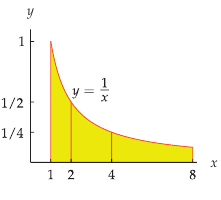
\includegraphics[scale=0.4]{pics/e_9.png}
\end{figure}
Each of these regions has the same area from the Area Stretch Theorem.
Generalizing the above in the case of \(2\) to \( c \)
\[ \text{area}\left(\frac{1}{x}, 1, c^{t}\right) = t*\text{area}\left(\frac{1}{x}, 1, c\right) \]

\subsection{Exponential Growth Revisited}
For compounding \(n\) times per year at an annual interest rate of \(r\), the amount after \(t\) years is given by
\[ P(t) = P_{0}\left(1+\frac{r}{n}\right)^{nt} \]
Assume \(n\) is large, let say once per hour \(n= 365*24 = 8760\), then we can use the approximation
\[ \left(1+\frac{r}{n}\right)^{n} \approx e^{r} \]
If we let \(n\) approach infinity, we get the formula for continuous compounding:
\[ P(t) = P_{0}e^{rt} \]

\subsection{Continuous growth rates}
If a population grows at a continuous rate of \(r\), then the population at time \(t\) is given by
\[ P(t) = P_{0}e^{rt} \]
where \(P_{0}\) is the initial population.

\subsection{Doubling Time}
The time it takes for a quantity to double in size is called the \textbf{doubling time}. For continuous growth, the doubling time \(T\) can be calculated using the formula:
\[ T = \frac{\ln(2)}{r}  \approx \frac{70}{R} \]
where \(R = 100*r \)  is the percentage continuous growth rate.
The annual interest rate needed for money to double in \(t\) years with continuous compounding is approximately
\[ r \approx \frac{\ln(2)}{t}   \implies R \approx \frac{70}{t} \]
percent.
